\Chapter{Weryfikacja i walidacja rozwiązania}\label{chapter:tests}
    Rozdział stanowi krytyczną ocenę wdrożonego systemu, podzieloną na dwie kluczowe perspektywy:
    \begin{itemize}
        \item \textbf{Testowanie funkcjonalności} --- weryfikacja, czy aplikacja działa zgodnie z założeniami projektowymi. Zawiera formalne scenariusze testowe oraz ich praktyczną realizację,
        \item \textbf{Analiza jakości wyniku} --- walidacja, czy wygenerowane plany lekcji są użyteczne i poprawne jakościowo. Obejmuje porównanie z planem ręcznym, analizę krytycznych przypadków oraz ewaluację kluczowego wskaźnika efektywności, liczby okienek nauczycieli.
    \end{itemize}

\section{Scenariusze testowe}

    \subsection{Scenariusz testowy generowania planu lekcji z określonymi parametrami}
        Scenariusz zaprezentowany w tabeli~\ref{tab:scenariusz_1} opisuje proces wygenerowania planu lekcji przy użyciu zaimplementowanego modułu optymalizacyjnego.

        \begin{table}[h!]
                \centering
                % \setlength{\tabcolsep}{8pt} % Default value: 6pt
                \caption{Generowanie planu lekcji z określonymi parametrami}\label{tab:scenariusz_1}
                \renewcommand{\arraystretch}{1.3} % 4efault value: 1
                \begin{tabular}{|p{0.25\textwidth}|p{0.70\textwidth}|}
                    \hline
                    \textbf{Scenariusz} & Generowanie planu lekcji z określonymi parametrami \\ \hline
                    
                    \textbf{Opis} & Test weryfikuje poprawność procesu generowania planu lekcji przy zadanej liczbie generacji oraz pełnym zestawie danych wejściowych. \\ \hline
                    
                    \textbf{Widok początkowy} & Strona główna \\ \hline
                    
                    \multirow{4}{*}{\textbf{Wymagania}}
                    & Wprowadzone zasoby: nauczyciele, klasy, sale, przedmioty \\
                    & Zdefiniowane wymagania główne dla każdej klasy \\
                    & Wprowadzone dostępności nauczycieli \\
                    & Zdefiniowane bloki przedmiotowe \\ \hline
                    
                    \multirow{3}{*}{\textbf{Kroki testowe}} 
                    & 1. Przejdź do widoku generowania planu lekcji \\
                    & 2. Wprowadź liczbę generacji \\
                    & 3. Wybierz dostępny zestaw ograniczeń \\
                    & 4. Uruchom proces generowania planu \\ \hline
                    
                    \textbf{Oczekiwany rezultat} &
                    System generuje kompletny plan lekcji zgodny ze wszystkimi ograniczeniami. System pokazuje użytkownikowi powiadomienie o zakończeniu procesu. \\ \hline
                \end{tabular}
            \end{table}

    \subsection{Scenariusz przeglądu planów lekcji}
        Scenariusz zaprezentowany w tabeli~\ref{tab:scenariusz_przegladu_planow} opisuje proces przeglądania istniejących planów lekcji wygenerowanych w systemie.

        \begin{table}[h!]
            \centering
            % \setlength{\tabcolsep}{8pt}
            \caption{Scenariusz przeglądu planów lekcji}\label{tab:scenariusz_przegladu_planow}\label{tab:scenariusz_2}
            \renewcommand{\arraystretch}{1.4}
            \begin{tabular}{|p{0.25\textwidth}|p{0.70\textwidth}|}
                \hline
                \textbf{Scenariusz} & Przegląd planów lekcji \\ \hline

                \textbf{Opis} & Test weryfikuje możliwość przeglądania wielu wygenerowanych planów lekcji oraz podglądu ich szczegółów z perspektywy klasy i nauczyciela. \\ \hline

                \textbf{Widok początkowy} & Strona główna \\ \hline

                \multirow{2}{*}{\textbf{Wymagania}}
                & Wprowadzone zasoby: nauczyciele, klasy, sale, przedmioty \\
                & W systemie dostępne są co najmniej dwa wygenerowane plany lekcji \\ \hline

                \multirow{4}{*}{\textbf{Kroki testowe}}
                & 1. Przejdź do widoku przeglądania planów lekcji \\
                & 2. Wybierz najnowszy dostępny plan \\
                & 3. Wyświetl plan lekcji dla wybranej klasy \\
                & 4. Wyświetl plan lekcji dla konkretnego nauczyciela \\ \hline

                \textbf{Oczekiwany rezultat} &
                Użytkownik może poprawnie przeglądać różne warianty planów lekcji oraz widoki szczegółowe, a system prezentuje dane zgodnie z zapisanym stanem. \\ \hline
            \end{tabular}
        \end{table}
            

    \subsection{Scenariusz importowania i edytowania wymagań głównych}
        Scenariusz zaprezentowany w tabeli~\ref{tab:scenariusz_3} opisuje proces masowego importu wymagań głównych oraz ich późniejszej ręcznej edycji.
        
        \begin{table}[h!]
            \centering
            % \setlength{\tabcolsep}{8pt}
            \caption{Scenariusz importowania i edytowania wymagań głównych}\label{tab:scenariusz_3}
            \renewcommand{\arraystretch}{1.4}
            \begin{tabular}{|p{0.25\textwidth}|p{0.70\textwidth}|}
                \hline
                \textbf{Scenariusz} & Importowanie i edytowanie wymagań głównych \\ \hline
                
                \textbf{Opis} & Test weryfikuje poprawność importu danych z pliku CSV oraz poprawność procesu edycji wymagań godzinowych dla klas i nauczycieli. \\ \hline
                
                \textbf{Widok początkowy} & Strona główna \\ \hline
                
                \multirow{2}{*}{\textbf{Wymagania}}
                & Wprowadzone zasoby: nauczyciele, klasy, przedmioty \\
                & Dostępny plik CSV zawierający wymagania główne \\ \hline
                
                \multirow{4}{*}{\textbf{Kroki testowe}}
                & 1. Przejdź do widoku dodawania wymagań głównych \\
                & 2. Wybierz odpowiednie zbiory zasobów \\
                & 3. Przeciągnij plik CSV do aplikacji \\
                & 4. Edytuj wymagania godzinowe dla wybranej klasy i nauczyciela \\
                & 5. Zapisz zmiany \\ \hline
                
                \textbf{Oczekiwany rezultat} &
                System poprawnie importuje dane z pliku CSV oraz umożliwia ich edycję i zapisanie nowych wartości. \\ \hline
            \end{tabular}
        \end{table}
        

    \subsection{Scenariusz edytowania dostępności nauczycieli}
        Scenariusz zaprezentowany w tabeli~\ref{tab:scenariusz_4} opisuje proces modyfikacji dostępności nauczycieli po wcześniejszym zdefiniowaniu wymagań głównych.
        
        \begin{table}[h!]
            \centering
            % \setlength{\tabcolsep}{8pt}
            \caption{Scenariusz edytowania dostępności nauczycieli}\label{tab:scenariusz_4}
            \renewcommand{\arraystretch}{1.4}
            \begin{tabular}{|p{0.25\textwidth}|p{0.70\textwidth}|}
                \hline
                \textbf{Scenariusz} & Edytowanie dostępności nauczycieli \\ \hline
                
                \textbf{Opis} & Test sprawdza możliwość modyfikacji godzin dostępności nauczycieli z poziomu odpowiedniego widoku systemu. \\ \hline
                
                \textbf{Widok początkowy} & Widok wprowadzania wymagań głównych \\ \hline
                
                \multirow{1}{*}{\textbf{Wymagania}}
                & Wprowadzone zasoby: nauczyciele \\ \hline
                
                \multirow{4}{*}{\textbf{Kroki testowe}}
                & 1. Rozwiń wstążkę nawigacji \\
                & 2. Przejdź do widoku dostępności nauczycieli \\
                & 3. Wybierz dostępny zbiór ograniczeń \\
                & 4. Edytuj dostępność wybranego nauczyciela \\
                & 5. Zapisz zmiany \\ \hline
                
                \textbf{Oczekiwany rezultat} &
                System zapisuje zmodyfikowane dane dostępności. System pokazuje powiadomienie o powodzeniu operacji \\ \hline
            \end{tabular}
        \end{table}

\section{Testowanie aplikacji}
    \subsection{Test generowania planu lekcji z określonymi parametrami}
        Test potwierdza poprawność procesu generowania planu zgodnie ze scenariuszem przedstawionym w tabeli~\ref{tab:scenariusz_1}.
        Jak widać na rysunku~\ref{fig:test_1} aplikacja pozwala użytkownikowi na zdefiniowanie liczby generacji i spełnia wszystkie wymagania.
        Kolejno wykonywane kroki to:
        \begin{itemize}
            \item przejście do widoku generowania planów lekcji,
            \item wpisywanie liczby generacji,
            \item wybieranie zbioru ograniczeń,
            \item uruchomienie procesu oraz otrzymane powiadomienie.
        \end{itemize}

        \begin{figure}[H]
            \centering
            \includegraphics[width=0.48\textwidth]{images/test1/krok1.png}
            \includegraphics[width=0.48\textwidth]{images/test1/krok2.png}
            \includegraphics[width=0.48\textwidth]{images/test1/krok3.png}
            \includegraphics[width=0.48\textwidth]{images/test1/krok4.png}
            \caption{Zrzuty ekranów wykonanych kroków dla scenariusza generowania planu lekcji}\label{fig:test_1}
        \end{figure}

    \subsection{Test przeglądania planów lekcji}
        Test weryfikuje realizację wymagań dotyczących wieloperspektywicznego wglądu w plan.
        Na rysunku~\ref{fig:test_2} przedstawiłem proces testowania tej funkcjonalności zgodnie ze scenariuszem przedstawionym w tabeli~\ref{tab:scenariusz_2}.
        Użytkownik kolejno:
        \begin{itemize}
            \item przechodzi do widoku przeglądania planów lekcji,
            \item wybiera najnowszy dostępny plan,
            \item wybiera perspektywę konkretnej klasy,
            \item wybiera perspektywę konkretnego nauczyciela.
        \end{itemize}

        \begin{figure}[H]
            \centering
            \includegraphics[width=0.48\textwidth]{images/test2/krok1.png}
            \includegraphics[width=0.48\textwidth]{images/test2/krok2.png}
            \includegraphics[width=0.48\textwidth]{images/test2/krok3.png}
            \includegraphics[width=0.48\textwidth]{images/test2/krok4.png}
            \caption{Zrzuty ekranów wykonanych kroków dla scenariusza przeglądania planów lekcji}\label{fig:test_2}
        \end{figure}

    \subsection{Test importowania i edytowania wymagań głównych}
        Test weryfikuje możliwość importowania wymagań głównych z pliku csv oraz możliwość ich modyfikowania.
        Na rysunku~\ref{fig:test_3} przedstawiłem kroki użytkownika testującego aplikację zgodnie ze scenariuszem przedstawionym w tabeli~\ref{tab:scenariusz_3}.
        Użytkownik kolejno:
        \begin{itemize}
            \item przychodzi do widoku dodawania wymagań głównych,
            \item wybiera odpowiednie zbiory zasobów,
            \item importuje plik csv,
            \item edytuje pojedyncze wymaganie główne,
            \item zapisuje zmiany i dostaje powiadomienie.
        \end{itemize}

        \newpage
        \begin{figure}[H]
            \centering
            \includegraphics[width=0.48\textwidth]{images/test3/krok1.png}
            \includegraphics[width=0.48\textwidth]{images/test3/krok2.png}
            \includegraphics[width=0.48\textwidth]{images/test3/krok3.png}
            \includegraphics[width=0.48\textwidth]{images/test3/krok4.png}
            \includegraphics[width=0.48\textwidth]{images/test3/krok5.png}
            \caption{Zrzuty ekranów wykonanych kroków dla scenariusza importowania i edytowania wymagań głównych}\label{fig:test_3}
        \end{figure}

    \newpage
    \subsection{Test edytowania dostępności nauczycieli}
        Test sprawdza poprawność modyfikacji dostępności zgodnie ze scenariuszem przedstawionym w tabeli~\ref{tab:scenariusz_4}.
        Rysunek~\ref{fig:test_3} przedstawia proces:
        \begin{itemize}
            \item wybrania widoku edytowania dostępności nauczycieli,
            \item wybierania odpowiedniego zbioru wymagań,
            \item edytowania dostępności pierwszych dwóch nauczycieli,
            \item zapisania wyniku oraz otrzymania powiadomienia o sukcesie operacji.
        \end{itemize}

        \begin{figure}[H]
            \centering
            \includegraphics[width=0.48\textwidth]{images/test4/krok1.png}
            \includegraphics[width=0.48\textwidth]{images/test4/krok2.png}
            \includegraphics[width=0.48\textwidth]{images/test4/krok3.png}
            \includegraphics[width=0.48\textwidth]{images/test4/krok4.png}
            \caption{Zrzuty ekranów wykonanych kroków dla scenariusza edytowania dostępności nauczycieli}\label{fig:test_4}
        \end{figure}


\section{Analiza jakości wyników generowania planu lekcji}
    \subsection{Omówienie danych wejściowych}
        Dane przekazane przez placówkę oświatową pochodzą z początkowej fazy procesu układania planu lekcji i uległy zmianom po uzyskaniu pełnych informacji o uczniach.
        W szczególności nie obejmują one lekcji wychowawczych (LW) oraz zajęć dodanych na końcowym etapie tworzenia planu (przykładowo EO, EZ, \dots).
        W konsekwencji nie było możliwe pełne zamodelowanie tych elementów ani uwzględnienie ich podczas optymalizacji planu.

        Istotnym ograniczeniem była również kwestia ochrony danych osobowych nauczycieli --- nie uzyskałem dostępu do imion i nazwisk, co uniemożliwiło identyfikację sytuacji, w których jeden nauczyciel prowadzi więcej niż jeden przedmiot.
        Tym samym nie można było zamodelować potencjalnych konfliktów wynikających z równoległego prowadzenia zajęć w różnych klasach przez tego samego nauczyciela.
    
    \subsection{Omówienie całego planu}
        Plan omówiony poniżej został wygenerowany używając osobnika przedstawionego w punkcie~\ref{subsection:przykladowy_ewolucyjny}.

        Ocenianie jakości wyników należy zacząć od analizy obciążeń dydaktycznych.
        Na rysunku~\ref{fig:dydaktyczne_nauczyciele_tygodniowo} przedstawiłem histogram wymaganej ygodniowej liczby godzin lekcyjnych do przeprowadzenia przez wszystkich nauczycieli $t\in\mathcal{T}$.
        Jest to wynik pierwszego etapu działania algorytmu.
        Analogicznie, na rysunku~\ref{fig:dydaktyczne_klasy_tygodniowo} zaprezentowałem histogram liczby obowiązkowych godzin lekcyjnych dla wszystkich klas $c\in\mathcal{C}$.

        \begin{figure}[H]
            \centering
            \begin{tikzpicture}
                \begin{axis}[
                    ybar,
                    bar width=1.5em,
                    xlabel={Obciążenie dydaktyczne $\boldsymbol{\beta}_t$},
                    x label style = {yshift=-1em},
                    ylabel={Liczba nauczycieli},
                    width=0.9\textwidth,
                    height=0.45\textwidth,
                    xtick=data,
                    ymin=0,
                    xticklabels={{[0,2]}, {[3,5]}, {[6,8]}, {[9,11]}, {[12,14]}, {[15,17]}, {[18,20]}, {[21,23]}, {[24,26]}, {[27,29]}, {[30,32]}, {[33,35]}},
                    xtick={0,1,2,3,4,5,6,7,8,9,10,11},
                    x tick label style={rotate=30, anchor=center, yshift=-0.9em, xshift=-0.45em}
                ]
                \addplot coordinates {
                    (0, 0+4)     % 1-2
                    (1, 3+1+4)   % 3-5
                    (2, 0+4+3)   % 6-8
                    (3, 1+2+3)   % 9-11
                    (4, 2+3+1)   % 12-14
                    (5, 2+2+4)   % 15-17
                    (6, 0+8+9)   % 18-20
                    (7, 5+1+1)   % 21-23
                    (8, 0+0+1)   % 24-26
                    (9, 0+0+0)   % 27-29
                    (10, 0+0+0)  % 30-32
                    (11, 0+1+0)  % 33-35
                };
                \end{axis}
            \end{tikzpicture}
            \caption{Histogram łącznych obciążeń dydaktycznych nauczycieli tygodniowo}\label{fig:dydaktyczne_nauczyciele_tygodniowo}
        \end{figure}

        \begin{figure}[H]
            \centering
            \begin{tikzpicture}
                \begin{axis}[
                    ybar,
                    bar width=1.5em,
                    xlabel={Obciążenie dydaktyczne $\boldsymbol{\beta}_c$},
                    ylabel={Liczba klas},
                    width=0.9\textwidth,
                    height=0.45\textwidth,
                    xtick=data,
                    ymin=0,
                    ytick={0, 1, 2, 3},
                ]
                \addplot coordinates {
                    (22, 1)
                    (23, 1)
                    (24, 0)
                    (25, 2)
                    (26, 1)
                    (27, 1)
                    (28, 1)
                    (29, 2)
                    (30, 1)
                    (31, 1)
                    (32, 2)
                    (33, 3)
                    (34, 1)
                    (35, 2)
                    (36, 2)
                };
                \end{axis}
            \end{tikzpicture}
            \caption{Histogram łącznych obciążeń dydaktycznych klas tygodniowo}\label{fig:dydaktyczne_klasy_tygodniowo}
        \end{figure}

        Przez anonimowość nazwisk nauczycieli, niektórzy zostali w modelu sztucznie rozbici na dwie lub trzy osoby.
        Powoduje to zaniżenie wymaganej tygodniowo liczby godzin od poszczególnych nauczycieli.

        Z kolei, ze względu na nieuwzględnienie części lekcji opisanych wcześniej, wymagana tygodniowa liczba godzin dla klas jest również sztucznie zaniżona.
        Mimo tego można zaobserwować, że niektóre klasy mają znacząco niższe obciążenia tygodniowe niż pozostałe.
        Wynika to przede wszystkim z faktu, że klasy maturalne realizują istotnie mniejszą liczbę zajęć niż, przykładowo, klasy pierwsze.

        Biorąc pod uwagę te obserwacje, możemy przejść do analizy dziennego obciążenia dydaktycznego.
        Na rysunkach~\ref{fig:dydaktyczne_nauczyciele_dni} oraz~\ref{fig:dydaktyczne_klasy_dni} przedstawiłem odpowiednio histogram dziennych obciążeń nauczycieli i klas,
        a na rysunkach~\ref{fig:funkcja_skladowa_ft} oraz~\ref{fig:funkcja_skladowa_fc} wartości funkcji $F_t$ i $F_c$ przed ich normalizacją w końcowej funkcji przystosowania opisanej w punkcie~\ref{subsction:przystosowanie}.
        
        \begin{figure}[H]
            \centering
            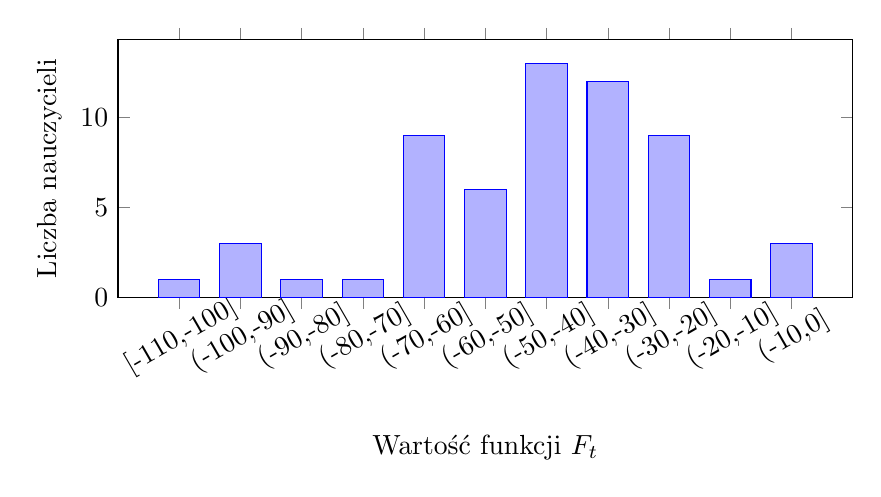
\begin{tikzpicture}
                \begin{axis}[
                    ybar,
                    bar width=1.5em,
                    xlabel={Wartość funkcji $F_t$},
                    x label style = {yshift=-1.2em},
                    ylabel={Liczba nauczycieli},
                    width=0.9\textwidth,
                    height=0.4\textwidth,
                    xtick={0,1,2,3,4,5,6,7,8,9,10},
                    xticklabels={{[-110,-100]},{(-100,-90]},{(-90,-80]},{(-80,-70]},{(-70,-60]},{(-60,-50]},{(-50,-40]},{(-40,-30]},{(-30,-20]},{(-20,-10]},{(-10,0]}},
                    x tick label style={rotate=30, anchor=center, yshift=-0.9em, xshift=-0.45em},
                    ymin=0
                ]
                \addplot coordinates {
                    (0, 1)
                    (1, 3)
                    (2, 1)
                    (3, 1)
                    (4, 9)
                    (5, 6)
                    (6, 13)
                    (7, 12)
                    (8, 9)
                    (9, 1)
                    (10, 3)
                };
                \end{axis}
            \end{tikzpicture}
            \caption{Histogram wartości składowej funkcji przystosowania $F_t$}\label{fig:funkcja_skladowa_ft}
        \end{figure}

        \begin{figure}[H]
            \centering
            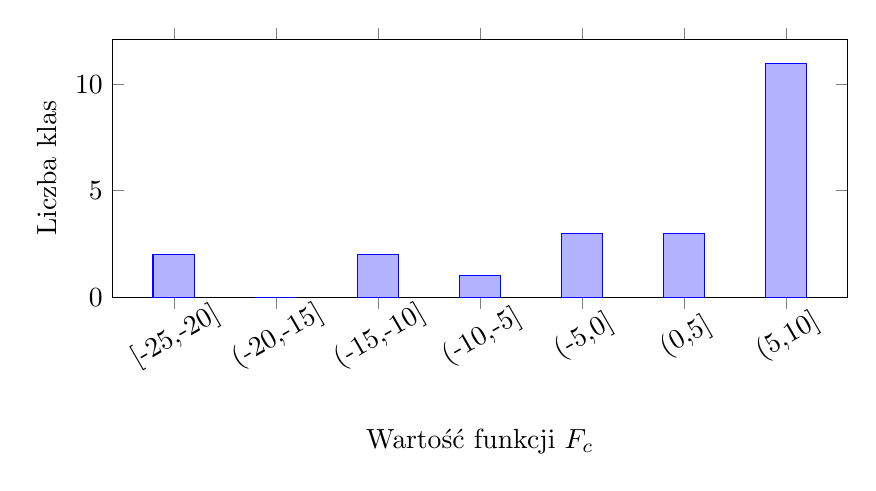
\begin{tikzpicture}
                \begin{axis}[
                    ybar,
                    bar width=1.5em,
                    xlabel={Wartość funkcji $F_c$},
                    x label style = {yshift=-1.2em},
                    ylabel={Liczba klas},
                    width=0.9\textwidth,
                    height=0.4\textwidth,
                    xtick={0,1,2,3,4,5,6},
                    xticklabels={{[-25,-20]},{(-20,-15]},{(-15,-10]},{(-10,-5]},{(-5,0]},{(0,5]},{(5,10]}},
                    x tick label style={rotate=30, anchor=center, yshift=-0.9em, xshift=-0.45em},
                    ymin=0
                ]
                \addplot coordinates {
                    (0, 2)
                    (1, 0)
                    (2, 2)
                    (3, 1)
                    (4, 3)
                    (5, 3)
                    (6, 11)
                };
                \end{axis}
            \end{tikzpicture}
            \caption{Histogram wartości składowej funkcji przystosowania $F_c$}\label{fig:funkcja_skladowa_fc}
        \end{figure}

        \begin{figure}[H]
            \centering
            \begin{tikzpicture}
                \begin{axis}[
                    ybar,
                    bar width=1.5em,
                    xlabel={Dzienne obciążenie dydaktyczne},
                    ylabel={Liczba dni o danym obciążeniu},
                    width=0.9\textwidth,
                    height=0.48\textwidth,
                    xtick=data,
                    ymin=0,
                ]
                \addplot coordinates {
                    (1,18)
                    (2,44)
                    (3,45)
                    (4,51)
                    (5,44)
                    (6,21)
                    (7,11)
                    (8,1)
                    (9,1)
                    (10,2)
                    (11,0)
                    (12,1)
                    (13,0)
                    (14,1)
                };
                \end{axis}
            \end{tikzpicture}
            \caption{Histogram dziennych obciążeń dydaktycznych nauczycieli}\label{fig:dydaktyczne_nauczyciele_dni}
        \end{figure}

        \begin{figure}[H]
            \centering
            \begin{tikzpicture}
                \begin{axis}[
                    ybar,
                    bar width=1.5em,
                    xlabel={Dzienne obciążenie dydaktyczne},
                    ylabel={Liczba dni o danym obciążeniu},
                    width=0.9\textwidth,
                    height=0.48\textwidth,
                    xtick=data,
                    ymin=0,
                ]
                \addplot coordinates {
                    (4,6)
                    (5,27)
                    (6,37)
                    (7,28)
                    (8,12)
                };
                \end{axis}
            \end{tikzpicture}
            \caption{Histogram dziennych obciążeń dydaktycznych klas}\label{fig:dydaktyczne_klasy_dni}
        \end{figure}

        W analizie nie biorę pod uwagę licznych dni wolnych od pracy nauczycieli, ponieważ jest to zamierzony efekt, osiągnięty dzięki modyfikacji funkcji przystosowania w algorytmie ewolucyjnym.
        Na rysunku~\ref{fig:funkcja_skladowa_ft} widać, że ocena rozłożenia obciążeń dydaktycznych nauczycieli nigdy nie przyjmuje wartości dodatnich.
        Wynika to z zastosowanych wag $\theta_T = 1$ i $\theta_G = 2$, które sprawiły, że algorytm w większym stopniu optymalizował obciążenia klas niż nauczycieli.
        W rezultacie pojawiły się także dwa przypadki, w których nauczyciel ma zaplanowane 12 lub 14 godzin zajęć w jednym dniu.
        Pomimo tego zdecydowana większość nauczycieli osiąga wyniki na poziomie około $F_t = -40$, co świadczy o poprawnej optymalizacji rozkładu ich obciążeń.

        Zastosowane wagi spowodowały jednocześnie, że rozkład obciążeń klas jest bardzo korzystny.
        Nie pojawiają się wartości skrajne ani nieakceptowalne.
        Na rysunku~\ref{fig:funkcja_skladowa_fc} widać, że przeważająca większość osiąga pozytywny wynik funkcji $F_c$ w przedziale od 5 do 10.
        Minimalne obciążenie widoczne na rysunku~\ref{fig:dydaktyczne_klasy_dni}, wynoszące 4 godziny, dotyczy klas maturalnych, które mają stosunkowo niską liczbę wymaganych godzin tygodniowo (22 lub 23).
        Wszystkie pozostałe wyniki mieszczą się w przedziale od 4 do 8 godzin dziennie, co umożliwia tworzenie praktycznych i realistycznych planów lekcji.
        
        Aby ocenić jakość wygenerowanych harmonogramów, przeanalizowałem także liczbę okienek nauczycieli w planie zoptymalizowanym pod kątem minimalizacji ich liczby oraz w planie, który jedynie spełnia wszystkie ograniczenia, lecz nie został poddany optymalizacji.
        Wyniki zestawiłem w tabeli~\ref{tab:statystyki_planow}.
        Ze względu na brak dostępu do szczegółowych danych dotyczących planu ułożonego ręcznie przez szkołę możliwe było jedynie porównanie wariantów wygenerowanych przez algorytm.

        \begin{table}[H]
            \centering
            % \setlength{\tabcolsep}{8pt} % Default value: 6pt
            \caption{Statystyki dla generowanych planów}\label{tab:statystyki_planow}
            \renewcommand{\arraystretch}{1.3} % 4efault value: 1
            \begin{tabular}{|p{0.45\textwidth}|c|c|c|c|c|c|}
                \hline
                \textbf{Dzień tygodnia} & Pon & Wt & Śr & Czw & Pt & Całościowo \\ \hline
                \textbf{Liczba bloków} & 132 & 133 & 133 & 135 & 140 & 673 \\ \hline
                \textbf{Liczba okienek przy minimalizacji} & 65 & 41 & 68 & 59 & 72 & 305 \\ \hline
                \textbf{Liczba okienek przy minimalizacji per nauczyciel} & 1.05 & 0.98 & 1.10 & 0.95 & 1.16 & 5.24 \\ \hline
                \textbf{Liczba okienek bez minimalizacji} & 172 & 157 & 141 & 139 & 133 & 742 \\ \hline
                \textbf{Liczba okienek bez minimalizacji per nauczyciel} & 2.77 & 2.53 & 2.27 & 2.24 & 2.15 & 11.96 \\ \hline
            \end{tabular}
        \end{table}

    
    \subsection{Omówienie szczególnych przypadków}
        Szczególnej analizie poddałem klasy o profilach łączonych, ponieważ to właśnie dla nich ręczne ułożenie planu jest najbardziej wymagające.
        W moim zbiorze danych klasa IIAC łączy profil psychologiczny z prawnym, co oznacza konieczność równoległego prowadzenia bloków lekcyjnych dotyczących obu ścieżek kształcenia.
        Wygenerowany plan lekcji dla tej klasy przedstawiłem na rysunku~\ref{fig:plan_IIBG}. 
        Dla porównania, na rysunku~\ref{fig:plan_IIBG_koper} zaprezentowałem plan opracowany ręcznie przez szkołę.

        \begin{figure}[H]
            \centering
            \includegraphics[width=0.9\textwidth]{images/plans/plan_IIBG_koper.png}
            \caption{Plan lekcji dla klasy IIAC stworzony przez szkołę}\label{fig:plan_IIBG_koper}
        \end{figure}
        \begin{sidewaysfigure}[p]
            \centering
            \includegraphics[width=\textwidth,height=\textheight,keepaspectratio]{images/plans/plan_IIBG.png}
            \caption{Wygenerowany plan lekcji dla klasy IIAC}\label{fig:plan_IIBG}
        \end{sidewaysfigure}

        Analizując wygenerowany plan można zauważyć, że algorytm poprawnie odwzorował wymagane bloki lekcyjne, takie jak jednoczesne prowadzenie języka biologii i wiedzy o społeczeństwie, a także prawidłowo przydzielił sale o specjalnym przeznaczeniu (sale gimnastyczne, pracownie informatyczne, \dots).
        Plan charakteryzuje się również równomiernym rozkładem obciążeń dydaktycznych w ciągu tygodnia.

        Kolejnym istotnym aspektem jest prawidłowe zaplanowanie zajęć prowadzonych jednocześnie dla wielu klas.
        Najczęściej występują tu bloki językowe obejmujące język francuski, niemiecki oraz rosyjski.
        Przykład takiego bloku, realizowanego w środy w pierwszym oraz drugim slocie czasowym, przedstawiłem na rysunku~\ref{fig:plan_blok}.

        \begin{sidewaysfigure}[p]
            \centering
            \includegraphics[width=\textwidth,height=\textheight,keepaspectratio]{images/plans/plan_blok_polaczony_2.png}
            \caption{Zestawienie środowych planów lekcji dla kolejno klas IIIA, IIIC, IIID, IIIF i IIIG}\label{fig:plan_blok}
        \end{sidewaysfigure}

        Wyniki potwierdzają wysoką skuteczność algorytmu --- średnio około pięciu okienek w ciągu całego tygodnia na nauczyciela można uznać za wynik satysfakcjonujący.

    \newpage
    \subsection{Wydajność generowania planu lekcji}
        Testy wydajnościowe przeprowadziłem na następującej konfiguracji sprzętowej:
        \begin{itemize}
            \item \textbf{procesor:} AMD Ryzen 7 2700X (16 wątków), 3.875 GHz,
            \item \textbf{karta graficzna:} AMD Radeon RX 7700 XT,
            \item \textbf{pamięć RAM:} 16GB,
            \item \textbf{system operacyjny}: Linux 6.17.9.arch1-1.
        \end{itemize}
        Przy czym warto zaznaczyć, że algorytm nie korzysta z karty graficznej.

        Czas generowania bloków lekcyjnych jest znikomy w porównaniu do pozostałych etapów (poniżej jednej sekundy).
        Średni czas działania algorytmu ewolucyjnego, obliczony na podstawie pięciu niezależnych prób, wyniósł 95 sekund.
        Następnie wygenerowanie pełnego planu zajęć wraz z minimalizacją liczby okienek zajęło 6 minut i 52 sekundy.

        Łączny czas potrzebny do uzyskania kompletnego planu lekcji dla rzeczywistych danych wyniósł zatem około 8.45 minuty.
        Jest to bardzo dobry rezultat, biorąc pod uwagę złożoność problemu, liczne zależności oraz obecność klas o profilach łączonych.
        Ponadto czas ten mieści się w wymaganym limicie 10 minut, określonym w wymaganiach niefunkcjonalnych systemu.